\section{Generazioni cellulari}
Nel corso degli anni, si sono susseguite diverse generazioni di tecnologie cellulari, che hanno apportato
notevoli cambiamenti alla loro architettura. Di seguito verranno presentati le principali caratteristiche
delle diverse generazioni cellulari, in modo tale da rendere di facile comprensione l'analisi dei meccanismi
di identificazione che verranno approfonditi nelle prossime sezioni.\\
Oltre ad elencare le principali caratteristiche di ogni generazione verranno analizzate nel dettaglio le specifiche  
dell'architettura di rete.
\begin{figure}[ht]
    \centering
    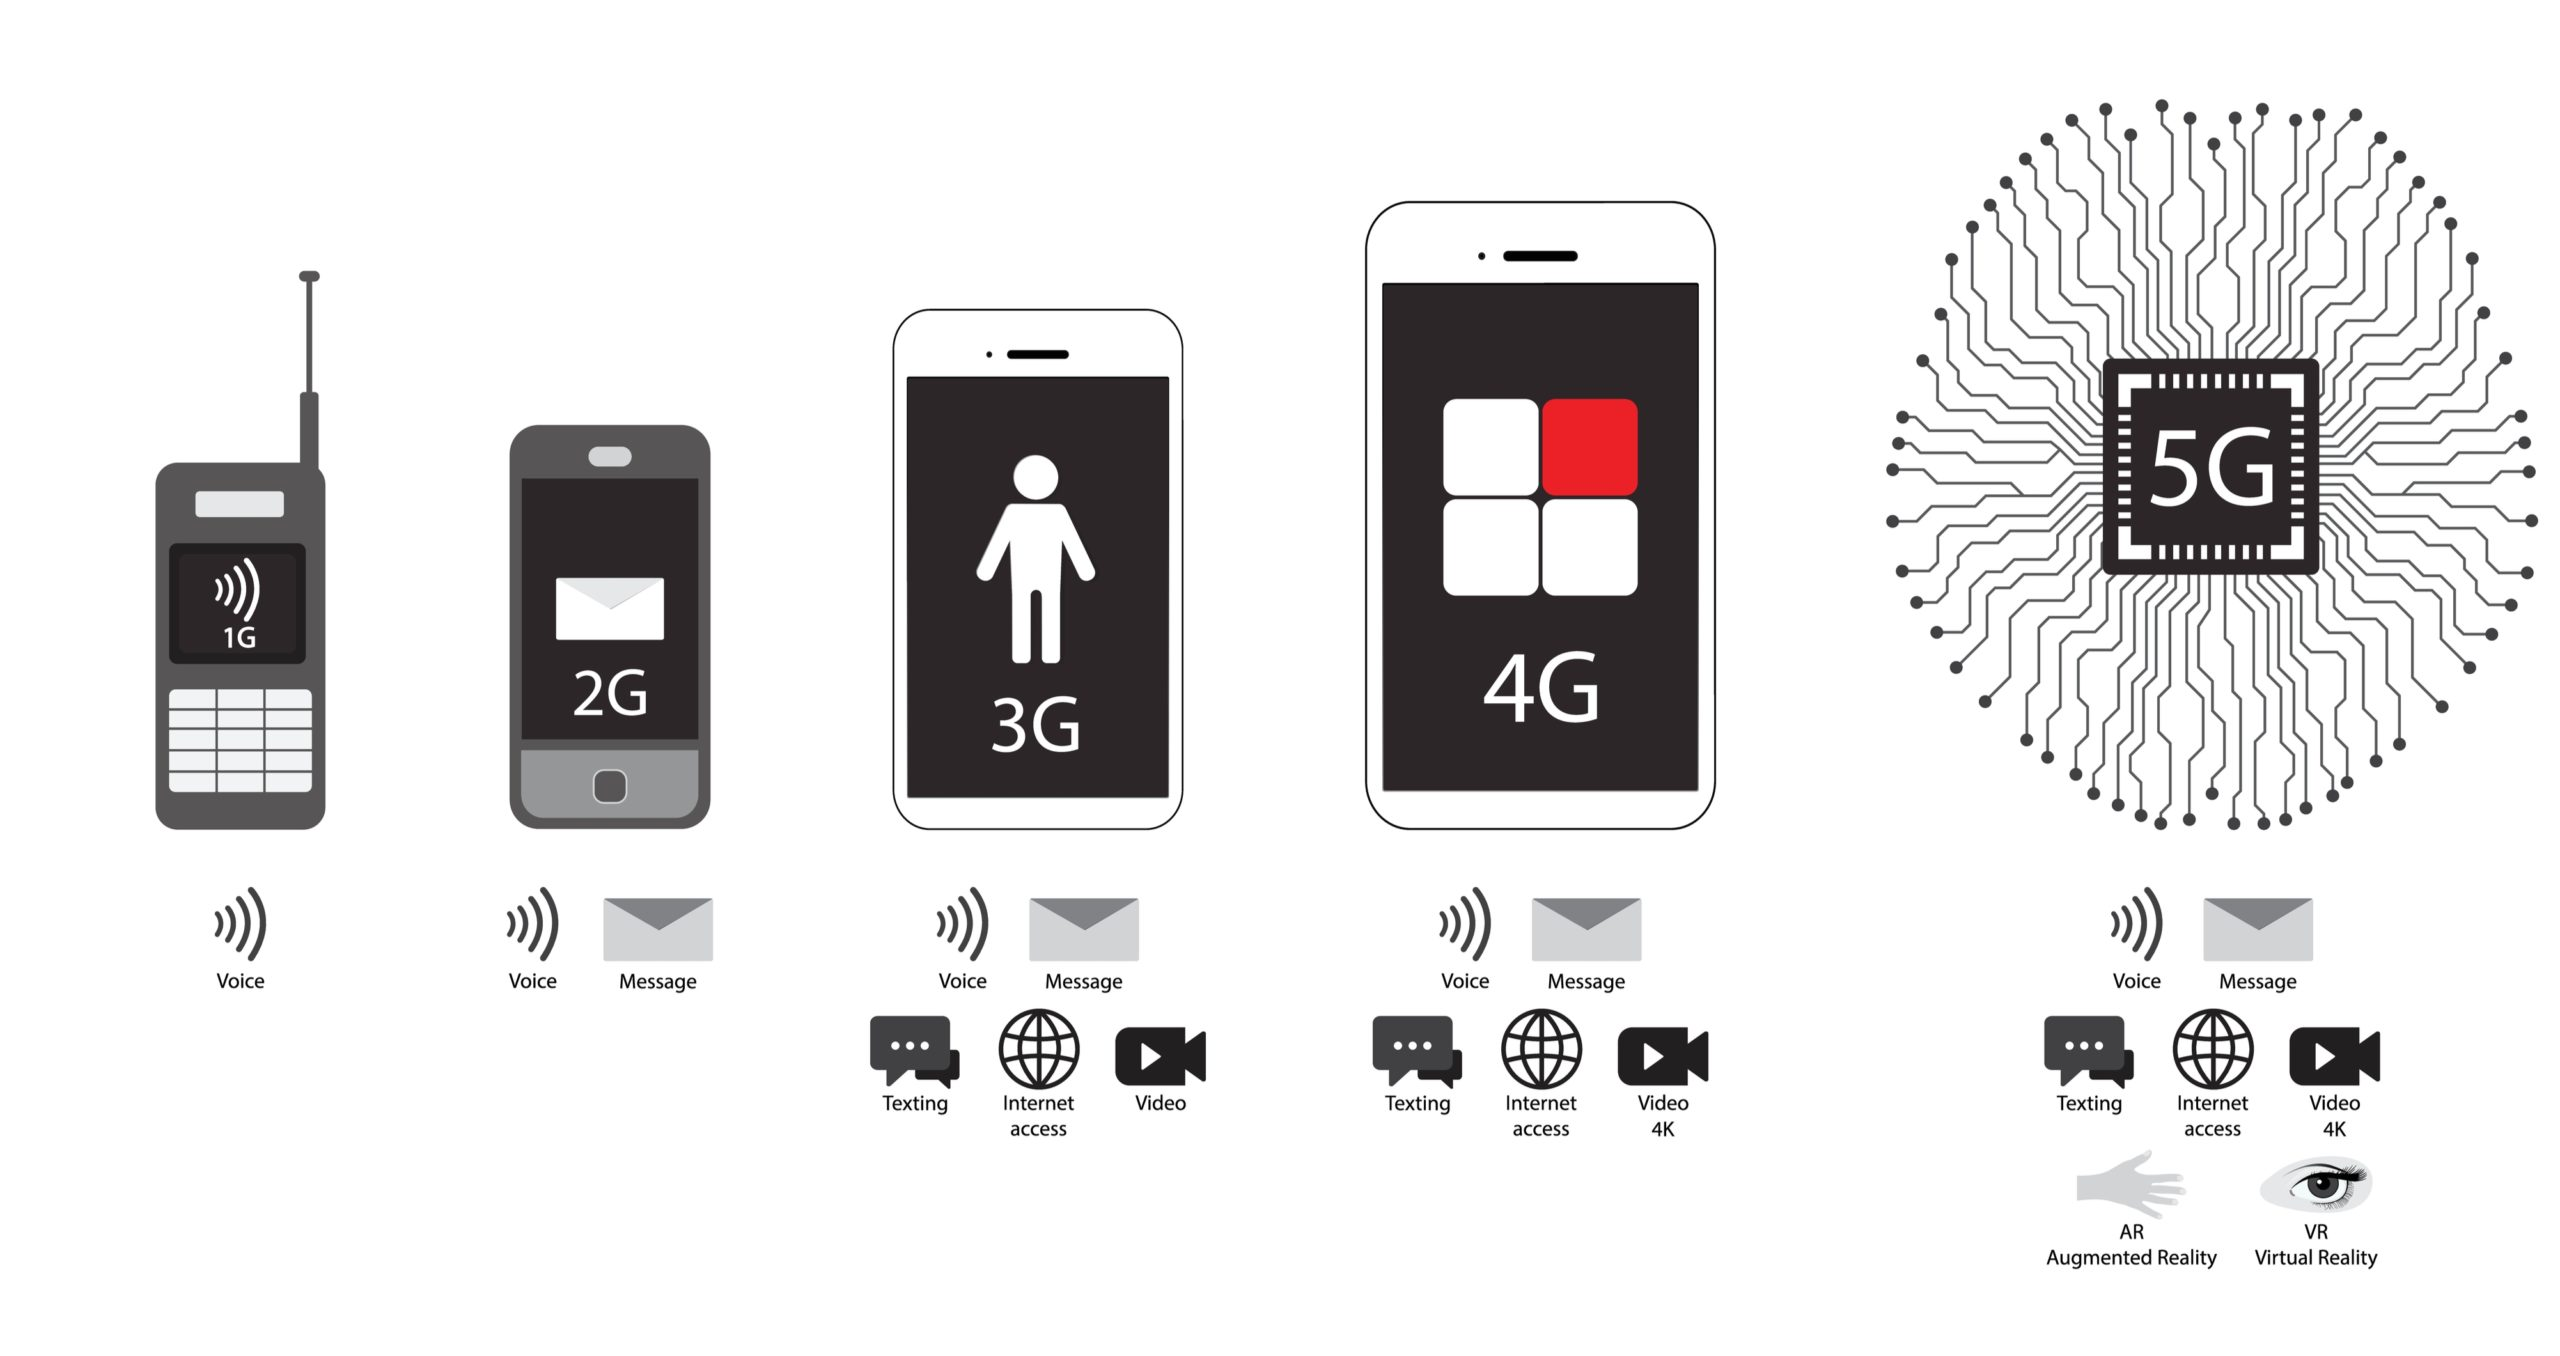
\includegraphics[width=0.7\textwidth]{images/generations-scheme.jpg}
    \caption{Schema delle generazioni cellulari}
\end{figure}

\subsection{1G}
La generazione 1G è uno dei primi standard di comunicazione cellulare. Il suo funzionamento era completamente analogico 
e ormai è stata rimpiazzata totalmente dalle generazioni digitali successive.\\
L'architettura di questa generazione è molto semplice, è composta da tre componenti principali:
\begin{itemize}
    \item Antenne per la trasmissione
    \item \textit{Mobile Telephone Switching Office} (MTSO)
    \item Unità mobile (cellulare)
\end{itemize}
\begin{figure}[ht]
    \centering
    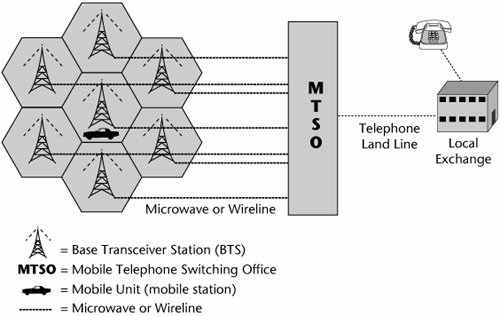
\includegraphics[width=0.7\textwidth]{images/1g.jpg}
    \caption{Architettura 1G}
\end{figure}
Si basava sulla \textit{frequency-division multiple access} (FDMA) in cui ogni dispositivo che si connetteva alla stazione radio
aveva assegnata una specifica sotto banda\cite{generations}.

\clearpage

\subsection{2G}
A differenza della prima generazione, la seconda introuduce per la prima volta una rete completamente digitale.
La seconda generazione cellulare è composta da diverse versioni che si sono susseguite nel corso degli anni aggiungendo nuove 
funzionalità.
Anche la sua architettura subisce delle modifiche, per questo verranno trattate in seguito.
\subsubsection{GSM}
Il GSM, ovvero \textit{Global System for Mobile Communications} è uno standard di seconda generazione che introuduce importanti novità.
Le principali caratteristiche introdotte sono:
\begin{itemize}
    \item Maggiori velocità di trasmissione
    \item Cifratura della comunicazione
    \item Introduzione di nuovi servizi come gli SMS
\end{itemize}
\begin{figure}[ht]
    \centering
    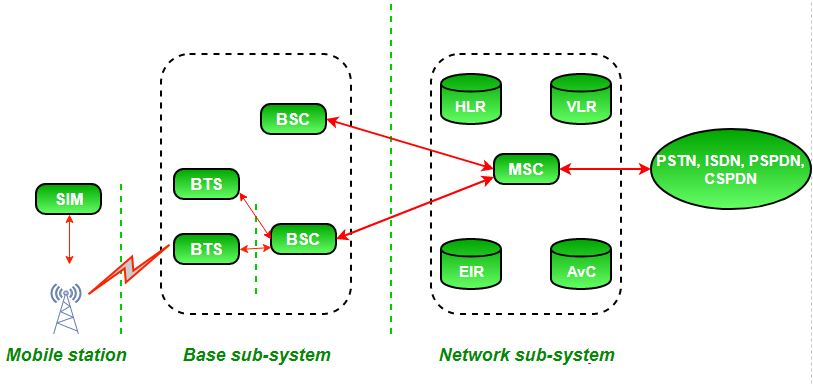
\includegraphics[width=0.7\textwidth]{images/2g-gsm.jpg}
    \caption{Architettura GSM}
\end{figure}
La sua architettura è composta da due macro aree: La BSS \textit{Base Station SubSystem} e la NSS \textit{Network SubSystem}.
Il BSS è l'insieme delle antenne ricevitori, rappresentano il primo collegamento con il MS.\\
Il MS si collega alla BS di riferimento, viene identificato tramite l'HLR \textit{Home Location Register}, ovvero un \textit{database} 
che contiene tutte le informazioni necessarie per la gestione dei \textit{subscribers}. Le chiamate e messaggi vengono smistati nella rete 
telefonica tramite il MSC \textit{Mobile Switching Centre}.
\subsubsection{GPRS}
La rete GPRS \textit{General Packet Radio Service} introduce per la prima volta un trasferimento dati a commutazione di pacchetto per rendere 
possibile l'utilizzo dei servizi \textit{internet} con il proprio dispositivo cellulare\cite{gsm-architecture}.
La sua architettura è la stessa di quella del GSM ma con dei componenti aggiuntivi che consentono la trasmissione dei pacchetti. 
Per esempio, il SGSN \textit{Serving GPRS Support Node} è un componente predisposto per la gestione dei dispositivi connessi alla rete.
\begin{figure}[ht]
    \centering
    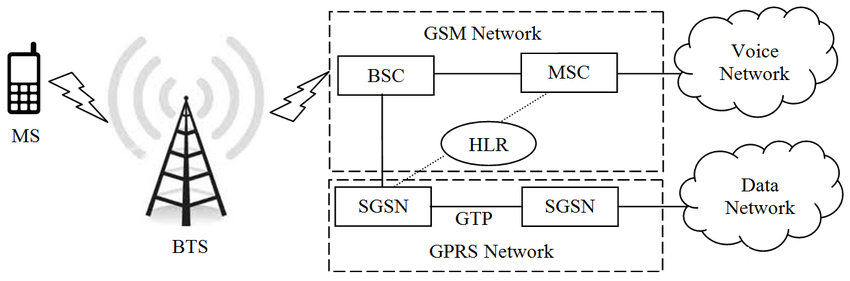
\includegraphics[width=0.7\textwidth]{images/2g-gprs.png}
    \caption{Architettura GPRS}
\end{figure}
\subsubsection{EDGE}
Evoluzione del GPRS che consente maggiori velocità, l'architettura resta invariata.

\clearpage

\subsection{3G}
\begin{figure}[ht]
    \centering
    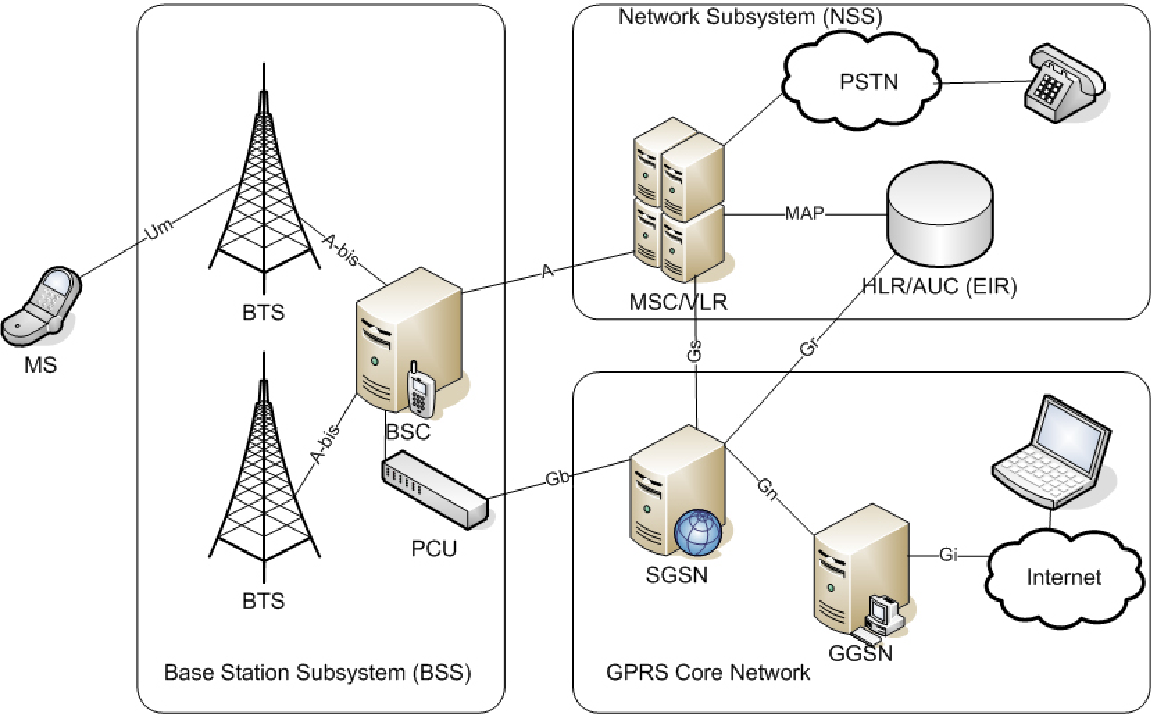
\includegraphics[width=0.7\textwidth]{images/3g-umts.png}
    \caption{Architettura UMTS}
\end{figure}

\subsubsection{UMTS}


\subsubsection{HSPA/HSPA+}

\clearpage

\subsection{4G}
\begin{figure}[ht]
    \centering
    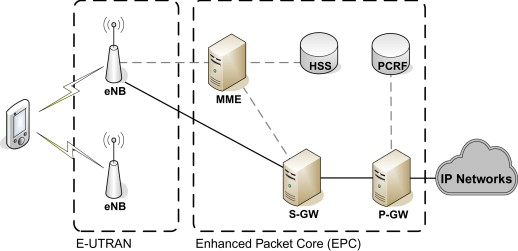
\includegraphics[width=0.8\textwidth]{images/4g-lte.jpg}
    \caption{Architettura LTE}
\end{figure}

\clearpage

\subsection{5G}
\begin{figure}[ht]
    \centering
    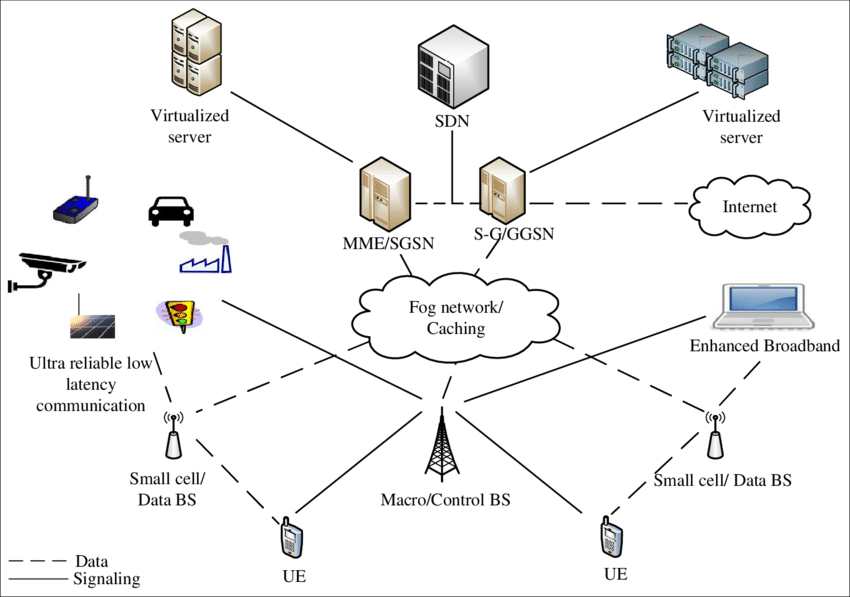
\includegraphics[width=0.7\textwidth]{images/5g.png}
    \caption{Architettura 5G}
\end{figure}